% LaTeX TikZ graphic for upsampling vs Conv2DTranspose
% Standalone example
\documentclass[tikz,border=10pt]{standalone}
\usepackage{tikz}

% Helper macro to draw a colored grid
% \grid{<x>}{<y>}{<colors comma>}

\begin{document}
% Simplified TikZ figure: 3x3 input -> 2x2 UpSampling2D -> 6x6 output

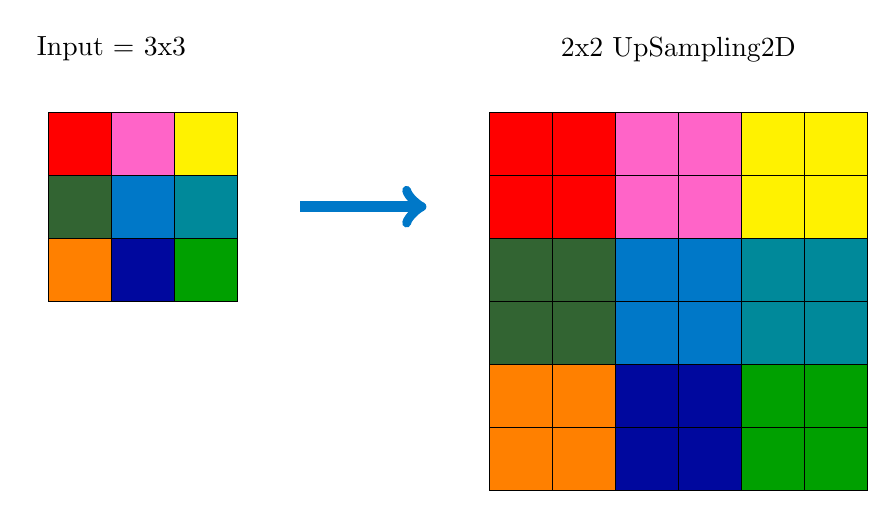
\begin{tikzpicture}[scale=0.8]

% Colors
\definecolor{pink}{RGB}{255,100,200} % pink
\definecolor{olive}{RGB}{50,100,50}   % olive
\definecolor{blue}{RGB}{0,120,200}   % blue
\definecolor{teal}{RGB}{0,170,120}   % teal
\definecolor{navy}{RGB}{0,137,154}     % navy
\definecolor{green}{RGB}{0,160,0}     % green
\definecolor{darkblue}{RGB}{0,8,158}

% === INPUT 3×3 ===
\node at (1,2) {Input = 3x3};

\draw[draw=black, fill=red] (0,0) rectangle ++(1,1);
\draw[draw=black, fill=pink] (1,0) rectangle ++(1,1);
\draw[draw=black, fill=yellow] (2,0) rectangle ++(1,1);

\draw[draw=black, fill=olive] (0,-1) rectangle ++(1,1);
\draw[draw=black, fill=blue] (1,-1) rectangle ++(1,1);
\draw[draw=black, fill=navy] (2,-1) rectangle ++(1,1);

\draw[draw=black, fill=orange] (0,-2) rectangle ++(1,1);
\draw[draw=black, fill=darkblue] (1,-2) rectangle ++(1,1);
\draw[draw=black, fill=green] (2,-2) rectangle ++(1,1);


% === Arrow ===
\draw[->, line width=4pt, blue] (4,-0.5) -- (6,-0.5);
\node at (10,2) {2x2 UpSampling2D};

% === Block ===
\draw[draw=black, fill=red] (7,0) rectangle ++(1,1);
\draw[draw=black, fill=red] (8,0) rectangle ++(1,1);
\draw[draw=black, fill=pink] (9,0) rectangle ++(1,1);
\draw[draw=black, fill=pink] (10,0) rectangle ++(1,1);
\draw[draw=black, fill=yellow] (11,0) rectangle ++(1,1);
\draw[draw=black, fill=yellow] (12,0) rectangle ++(1,1);

\draw[draw=black, fill=red] (7,-1) rectangle ++(1,1);
\draw[draw=black, fill=red] (8,-1) rectangle ++(1,1);
\draw[draw=black, fill=pink] (9,-1) rectangle ++(1,1);
\draw[draw=black, fill=pink] (10,-1) rectangle ++(1,1);
\draw[draw=black, fill=yellow] (11,-1) rectangle ++(1,1);
\draw[draw=black, fill=yellow] (12,-1) rectangle ++(1,1);

\draw[draw=black, fill=olive] (7,-2) rectangle ++(1,1);
\draw[draw=black, fill=olive] (8,-2) rectangle ++(1,1);
\draw[draw=black, fill=blue] (9,-2) rectangle ++(1,1);
\draw[draw=black, fill=blue] (10,-2) rectangle ++(1,1);
\draw[draw=black, fill=navy] (11,-2) rectangle ++(1,1);
\draw[draw=black, fill=navy] (12,-2) rectangle ++(1,1);

\draw[draw=black, fill=olive] (7,-3) rectangle ++(1,1);
\draw[draw=black, fill=olive] (8,-3) rectangle ++(1,1);
\draw[draw=black, fill=blue] (9,-3) rectangle ++(1,1);
\draw[draw=black, fill=blue] (10,-3) rectangle ++(1,1);
\draw[draw=black, fill=navy] (11,-3) rectangle ++(1,1);
\draw[draw=black, fill=navy] (12,-3) rectangle ++(1,1);

\draw[draw=black, fill=orange] (7,-4) rectangle ++(1,1);
\draw[draw=black, fill=orange] (8,-4) rectangle ++(1,1);
\draw[draw=black, fill=darkblue] (9,-4) rectangle ++(1,1);
\draw[draw=black, fill=darkblue] (10,-4) rectangle ++(1,1);
\draw[draw=black, fill=green] (11,-4) rectangle ++(1,1);
\draw[draw=black, fill=green] (12,-4) rectangle ++(1,1);

\draw[draw=black, fill=orange] (7,-5) rectangle ++(1,1);
\draw[draw=black, fill=orange] (8,-5) rectangle ++(1,1);
\draw[draw=black, fill=darkblue] (9,-5) rectangle ++(1,1);
\draw[draw=black, fill=darkblue] (10,-5) rectangle ++(1,1);
\draw[draw=black, fill=green] (11,-5) rectangle ++(1,1);
\draw[draw=black, fill=green] (12,-5) rectangle ++(1,1);

\end{tikzpicture}
\end{document}
